\documentclass{article}

\usepackage[a4paper,margin=2.5cm]{geometry}
\usepackage{tikz}
\usepackage{amsmath}
\usepackage{fancyhdr}
\usepackage{hyperref}
\usepackage{float}
\usepackage{subcaption}
\usepackage{forest}
\usepackage{xcolor}
\usepackage{multirow}
\usepackage[shortlabels]{enumitem}

\forestset{el/.style={edge label={node [pos=1,above,outer sep=3pt] {$#1$} }}}

\title{\vspace{-2cm}ECON20005 Assignment 1}
\date{\today}
\author{Lucas Fern (1080613)\\Friday 12:00pm Tutorial}

\begin{document}
\maketitle
\paragraph{Notation Convention} In this assignment $(\mbox{ANZ}, \mbox{ANZ})$ represents a strategy where the player chooses ANZ in in two subgames. Sets of strategies appear in curly braces - \{\}.
\section*{Question 1: Marriage and banking}
\subsection*{1.1}
\begin{center}
    \begin{forest}
        for tree={circle,s sep = 35pt,calign=center}
        [Tommy,
         [Gina,edge={->, red, line width=1.5pt},edge label={node[above left,midway,font=\scriptsize]{ANZ}}
          [{(22, 25)},edge={->, red, line width=1.5pt},edge label={node[midway,above left,font=\scriptsize]{ANZ}}]
          [{(18, $M^2$)},edge={->, blue, line width=1pt},edge label={node[midway,above right,font=\scriptsize]{NAB}}]
         ]
         [Gina,edge={->, blue, line width=1.5pt},edge label={node[midway,above right,font=\scriptsize]{NAB}}
          [{(18, 25)},edge={->, red, line width=1pt},edge label={node[midway,above left,font=\scriptsize]{ANZ}}]
          [{(22, $M^2$)},edge={->, blue, line width=1.5pt},edge label={node[midway,above right,font=\scriptsize]{NAB}}]
         ]
        ]
    \end{forest}
\end{center}

\subsection*{1.2}
\begin{enumerate}[label=\textbf{\alph*}.]
    \item Tommy and Gina.
    \item \mbox{NAB} and \mbox{ANZ}.
    \item It is a sequential game.
    \item There is perfect information.
\end{enumerate}

\subsection*{1.3}
Tommy has the set of strategies $\{(\mbox{ANZ}), (\mbox{NAB})\}$.\\[2mm]
Gina has $\{(\mbox{ANZ}, \mbox{ANZ}), (\mbox{ANZ}, \mbox{NAB}), (\mbox{NAB}, \mbox{ANZ}),(\mbox{NAB}, \mbox{NAB})\}$.

\subsection*{1.4}
For $M\leq 5$, Gina's strategy is $\{(\mbox{ANZ}, \mbox{ANZ})\}$, and for $M\geq 5$ her strategy is $\{(\mbox{NAB}, \mbox{NAB})\}$. By pruning the tree we resolve that Tommy's strategy is $\{(\mbox{ANZ})\}$ for $M\leq 5$ and $\{(\mbox{NAB})\}$ for $M\geq 5$.\\[2mm]
Therefore the equilibrium strategies for $M\leq 5$ are Tommy: $\{(\mbox{ANZ})\}$, and Gina: $\{(\mbox{ANZ}, \mbox{ANZ})\}$. The equilibrium path is $\mbox{ANZ} \rightarrow \mbox{ANZ}$, and the equilibrium strategies are illustrated with {\color{red}red} arrows in Question 1.1.\\[2mm]
For $M\geq 5$ the equilibrium strategies are Tommy: $\{(\mbox{NAB})\}$, and Gina: $\{(\mbox{NAB}, \mbox{NAB})\}$. Here the equilibrium path is $\mbox{NAB} \rightarrow \mbox{NAB}$, and the equilibrium strategies are illustrated with {\color{blue}blue} arrows.

\subsection*{1.5} In this game table, Tommy's best action for each of Gina's options is \underline{\textbf{underlined and bold}}. Gina's best actions for $M<5$ are highlighted {\color{red}red}, and {\color{blue}blue} for $M>5$. For $M<5$ the equilibrium outcome is that they both choose ANZ, and for $M>5$ they both choose NAB. Again, at $M=5$ both of these options are Nash equilibria.\\
\begin{table}[ht]
    \centering
    \begin{tabular}{cccc}
                                                    &                          & \multicolumn{2}{c}{Gina}                                     \\ \cline{3-4} 
                                                    & \multicolumn{1}{c|}{}    & \multicolumn{1}{c|}{ANZ}    & \multicolumn{1}{c|}{NAB}       \\ \cline{2-4} 
        \multicolumn{1}{c|}{\multirow{2}{*}{Tommy}} & \multicolumn{1}{c|}{ANZ} & \multicolumn{1}{c|}{\underline{\textbf{22}}, {\color{red}25}} & \multicolumn{1}{c|}{18, {\color{blue}$M^2$}} \\ \cline{2-4} 
        \multicolumn{1}{c|}{}                       & \multicolumn{1}{c|}{NAB} & \multicolumn{1}{c|}{18, {\color{red}25}} & \multicolumn{1}{c|}{\underline{\textbf{22}}, {\color{blue}$M^2$}} \\ \cline{2-4} 
    \end{tabular}
\end{table}
These equilibria are subgame perfect in all situations as neither player can unilaterally deviate from the equilibrium strategies to secure a higher payoff.
\subsection*{1.6}
At $M=5$ Gina is indifferent between the banks as she receives an equal payoff of 25 regardless of her choice. The two equilibrium strategies in this case are:
\begin{itemize}
    \item Tommy: $\{(\mbox{ANZ})\}$, and Gina: $\{(\mbox{ANZ}, \mbox{ANZ})\}$; and
    \item Tommy: $\{(\mbox{NAB})\}$, and Gina: $\{(\mbox{NAB}, \mbox{NAB})\}$.
\end{itemize}
Either of these strategies result in an identical payoff of $(22,25)$ at $M=5$ and there is no incentive for either player to deviate from these strategies meaning they are both Subgame Perfect Nash Equilibria.

\section*{Question 2: Iteratively eliminating dominated strategies}
\subsection*{2.1} Iterative elimination of dominated strategies results in the removal of the rows shown here:
\begin{center}
    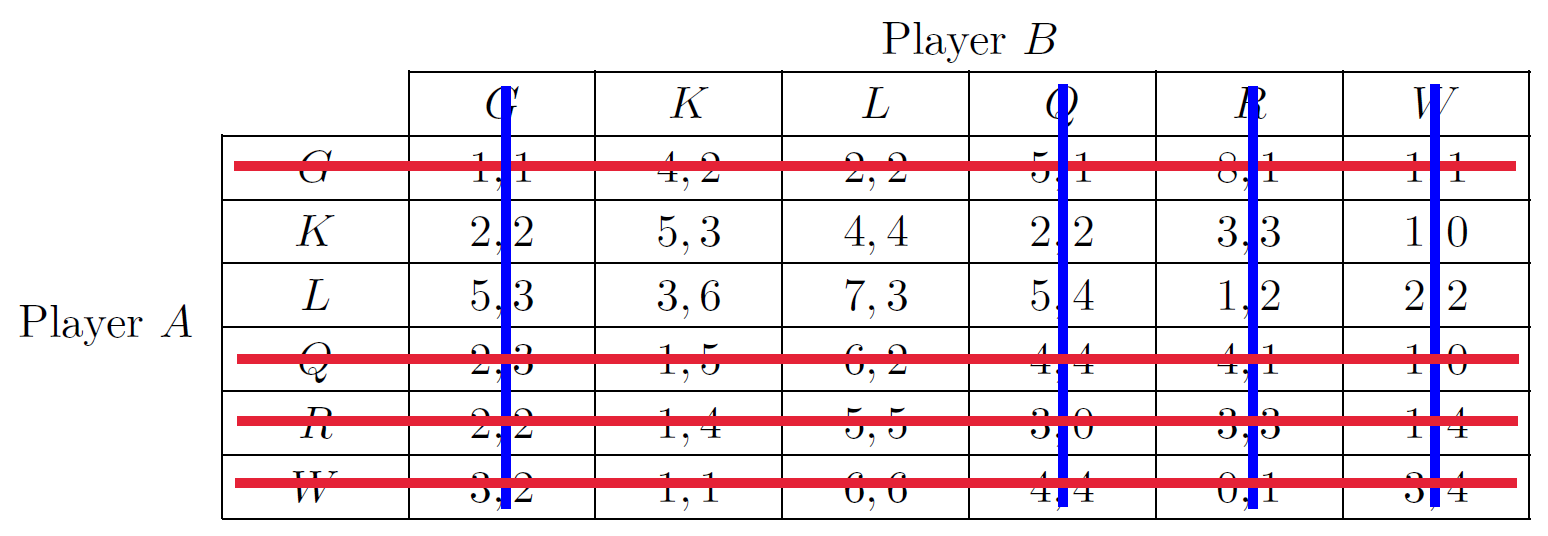
\includegraphics[width=0.7\linewidth]{iterative-elimination.png}
\end{center}
This results in the normal form game:
\begin{table}[h!]
    \centering
    \begin{tabular}{cccc}
                                                   &                        & \multicolumn{2}{c}{Player B}                          \\ \cline{3-4} 
                                                   & \multicolumn{1}{c|}{}  & \multicolumn{1}{c|}{K}    & \multicolumn{1}{c|}{L}    \\ \cline{2-4} 
    \multicolumn{1}{c|}{\multirow{2}{*}{Player A}} & \multicolumn{1}{c|}{K} & \multicolumn{1}{c|}{{\color{red}5}, 3} & \multicolumn{1}{c|}{4, {\color{blue}4}} \\ \cline{2-4} 
    \multicolumn{1}{c|}{}                          & \multicolumn{1}{c|}{L} & \multicolumn{1}{c|}{3, {\color{blue}6}} & \multicolumn{1}{c|}{{\color{red}7}, 3} \\ \cline{2-4} 
    \end{tabular}
\end{table}

\subsection*{2.2}
In the table that emerges from Question 2.1 each players' best responses have been highlighted. From this we can see that there are \textit{no} pure-strategy Nash equilibria.

\subsection*{2.3}
The cell corresponding to both players choosing K has a sum of payoffs $5+3 = 8$, the cell with both players choosing L has sum of payoffs $7+3 = 10$. $8 \neq 10$, so this is not a zero sum game.

\newpage
\section*{Question 3: Paul and Ringo take a vacation}
\subsection*{3.1}
\textbf{Extensive form:}
\begin{figure}[H]
    \centering
    \begin{forest}
        for tree={circle,s sep = 35pt,calign=center}
        [Paul,
         [Ringo,edge={->, red, line width=1.5pt},name=rleft,edge label={node[above left,midway,font=\scriptsize]{Gold Coast}}
          [{(5, 3)},edge={->, red, line width=1.5pt},edge label={node[midway,above left,font=\scriptsize]{Gold Coast}}]
          [{(-2, -2)},edge={->, blue, line width=1pt},edge label={node[midway,above right,font=\scriptsize]{Queenstown}}]
         ]
         [Ringo,edge={->, blue, line width=1.5pt},name=rright, edge label={node[midway,above right,font=\scriptsize]{Queenstown}}
          [{(-2, -2)},edge={->, red, line width=1pt},edge label={node[midway,above left,font=\scriptsize]{Gold Coast}}]
          [{(1, 6)},edge={->, blue, line width=1.5pt},edge label={node[midway,above right,font=\scriptsize]{Queenstown}}]
         ]
        ]
        \draw[dashed] (rleft) to[out=0,in=180] (rright);
    \end{forest}
\end{figure}
\noindent \textbf{Normal form:}
\begin{table}[h!]
    \centering
    \begin{tabular}{cccc}
                                                   &                                 & \multicolumn{2}{c}{Ringo}                                         \\ \cline{3-4} 
                                                   & \multicolumn{1}{c|}{}           & \multicolumn{1}{c|}{Gold Coast} & \multicolumn{1}{c|}{Queenstown} \\ \cline{2-4} 
        \multicolumn{1}{c|}{\multirow{2}{*}{Paul}} & \multicolumn{1}{c|}{Gold Coast} & \multicolumn{1}{c|}{\textbf{5, 3}}       & \multicolumn{1}{c|}{-2, -2}     \\ \cline{2-4} 
        \multicolumn{1}{c|}{}                      & \multicolumn{1}{c|}{Queenstown} & \multicolumn{1}{c|}{-2, -2}     & \multicolumn{1}{c|}{\textbf{1, 6}}       \\ \cline{2-4} 
    \end{tabular}
\end{table}

\subsection*{3.2} Using best response analysis on the Normal Form game table shows that two Nash equilibria exist, these are when either both players choose `Gold Coast', or both players choose `Queenstown'. These equilibria are illustrated on the extensive form game tree in {\color{red}red} and {\color{blue}blue} respectively, note that Ringo is forced to make the same choice at each of his decision nodes since it is a simultaneous game.

\subsection*{3.3} The game does not have a focal point since Paul gets a higher payoff in the Gold Coast equilibrium than in the Queenstown equilibrium, and the opposite is true for Ringo.

\subsection*{3.4} The extensive form of this game is as follows:
\begin{figure}[H]
    \centering
    \begin{forest}
        for tree={circle,s sep = 35pt,calign=center}
        [Paul,
         [Ringo,edge={->, red, line width=1.5pt},edge label={node[above left,midway,font=\scriptsize]{Gold Coast}}
          [{(5, 3)},edge={->, red, line width=1.5pt},edge label={node[midway,above left,font=\scriptsize]{Gold Coast}}]
          [{(-2, -2)},edge label={node[midway,above right,font=\scriptsize]{Queenstown}}]
         ]
         [Ringo, edge label={node[midway,above right,font=\scriptsize]{Queenstown}}
          [{(-2, -2)},edge label={node[midway,above left,font=\scriptsize]{Gold Coast}}]
          [{(1, 6)},edge={->, red, line width=1.5pt},edge label={node[midway,above right,font=\scriptsize]{Queenstown}}]
         ]
        ]
    \end{forest}
\end{figure}
\noindent The path of the SPNE is Gold Coast $\rightarrow$ Gold Coast, Paul's SPNE strategy is \{Gold Coast\}, and Ringo's is \{Gold Coast, Queenstown\}. This is illustrated on the game tree in {\color{red}red}.\\[2mm]
The game has a first mover advantage as Paul is able to make Ringo choose Gold Coast (Paul's maximum payoff) since it is detrimental to Ringo to disagree with Paul's decision.

\subsection*{3.5} \paragraph{Note} To save space in this question Gold Coast and Queenstown are abbreviated GC and QT respectively.\\[2mm]
The extensive form game is the following, where each players equilibrium strategies are highlighted in {\color{red}red}.
\begin{figure}[H]
    \centering
    \begin{forest}
        for tree={circle,s sep = 20pt,calign=center}
        [Ringo,
        [Paul, edge={->, red, line width=1.5pt}, edge label={node[above left,midway,font=\scriptsize]{Purchase \textbf{Extreme} Sports Pack}}
        [Ringo,edge label={node[above left,midway,font=\scriptsize]{GC}}
         [{(-2, 5)},edge label={node[midway,above left,font=\scriptsize]{GC}}]
         [{(8, -2)},edge={->, red, line width=1.5pt}, edge label={node[midway,above right,font=\scriptsize]{QT}}]
        ]
        [Ringo, edge={->, red, line width=1.5pt}, edge label={node[midway,above right,font=\scriptsize]{QT}}
         [{(-7, -2)},edge label={node[midway,above left,font=\scriptsize]{GC}}]
         [{(10, 1)},edge={->, red, line width=1.5pt}, edge label={node[midway,above right,font=\scriptsize]{QT}}]
        ]
       ]
       [Paul, edge label={node[above right,midway,font=\scriptsize]{Don't Purchase \textbf{Extreme} Sports Pack}}
       [Ringo,edge={->, red, line width=1.5pt},edge label={node[above left,midway,font=\scriptsize]{GC}}
        [{(3, 5)},edge={->, red, line width=1.5pt}, edge label={node[midway,above left,font=\scriptsize]{GC}}]
        [{(-2, -2)},edge label={node[midway,above right,font=\scriptsize]{QT}}]
       ]
       [Ringo, edge label={node[midway,above right,font=\scriptsize]{QT}}
        [{(-2, -2)},edge label={node[midway,above left,font=\scriptsize]{GC}}]
        [{(6, 1)},edge={->, red, line width=1.5pt}, edge label={node[midway,above right,font=\scriptsize]{QT}}]
       ]
      ]
     ]
    \end{forest}
\end{figure}
\noindent In this situation, the SPNE path is `Purchase \textbf{Extreme} Sports Pack' $\rightarrow$ Queenstown $\rightarrow$ Queenstown. The players equilibrium strategies are:
\begin{itemize}
    \item Ringo: \{(Purchase \textbf{Extreme} Sports Pack, QT, QT, GC, QT)\}; and,
    \item Paul: \{(QT, GC)\}.
\end{itemize}

\subsection*{3.6}
The sports pack \textit{can} be seen as a commitment device, this works because when it comes to Paul's decision, if Ringo has the sports pack, Paul knows that Ringo will be happy to go to Queenstown by himself. This makes Paul pick Queenstown too so that they can enjoy the payoff from both going to the same location.
\end{document}